Of course in this case too we are talking about variable length objects, not just text strings.
We store them with an array of pointers of sorted strings.
We define $N$ as the total length of strings and $\sigma = |\Sigma|$ as the alphabet size, then we will use $\$$ as the smallest symbol in the lexicographic order and $\#$ as the biggest one.

The problem is: given a pattern $P[1, p]$ we want to find (count or retrieve) all the occurrences of $P$ as prefix of the dictionary of strings.
Hashes can't be used since we are searching for a partial part of the key.

Let's suppose that our pattern is $P = te$ we can notice that:
\begin{itemize}
    \item all the strings that matches the prefix $P$ are contiguous in the array, since it's sorted;
    \item the starting position is the lexicographic position of $P\$$;
    \item the ending position is the lexicographic position of $P\#$.
\end{itemize}

As we are working we can already say that:
\begin{itemize}
    \item count is the subtraction end to start, and it's $O(1)$ operation;
    \item retrieve is proportional to the occurrences.
\end{itemize}
when we already know ending and starting positions.
We just need to find those positions.

\section{Binary search}
We can use binary search:
\begin{itemize}
    \item $O(p log_2 n)$ time;
    \item $O(\frac{p}{B}log_2 n)$ I/Os;
    \item $O(Nlog_2 \sigma + n log_2 N)$ bits space.
\end{itemize}


\subsection{Improve locality}
To boost performance instead of asking to the system to allocate single strings we ask for the whole memory and store strings one after the other.
Then instead of an array of pointers we can use an array $A$ of offsets from the start of the array.

Now whenever I restrict to a part of the array $A$ I restrict also on a part of memory, that can save I/Os in retrieve because we can exploit locality of reference.
So we achieve:
$$
    O \left( \frac{P}{B} log_2 \frac{N}{B} \right)
$$
I/Os.

Moreover now we exploit the fact that the array is sorted so common prefixes are near inside this version.

\section{Front coding}
Using front coding we can gain a 50\% compression on average, it states that you store strings with $< \text{length shared prefix}, \text{remaining suffix}>$:

Eg: alcatraz, alcool, alcyone, alu, box: $<0, alcatraz>, <3, ool>, \_, <0, box>$

But now how big we create the number to store the length?
Engineering the store we use a single byte which can store from 0 to 255, and if the length is more we allocate 2 more bytes to store the excess.

\subsection{Front coding and 2-level indexing}
In prefix search this storing is useless since if we want to random access we should go backward until we find the actual real prefix of the random element we are accessing which could lead us even to the first string.

What we can do to make it useful is to split the strings inside some blocks and front-encode each block.
Then on retrieve we start from the first string of the block and go on to rebuild the entire block:
\begin{itemize}
    \item first string is stored uncompressed for each block;
    \item we can build $A$ using pointers to the block start.
\end{itemize}
\begin{figure}[H]
    \centering
    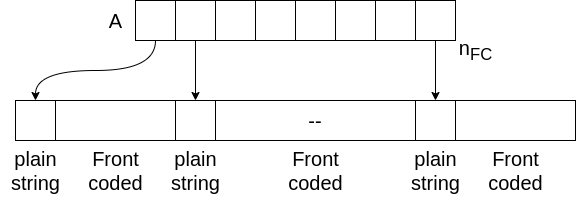
\includegraphics[width=250px]{images/8_Prefix_search/prefix_search_two_level_indexing.png}
\end{figure}

So in search we have:
$$
    \frac{P}{B}log_2 \frac{FC(D)}{B}
$$
I/Os for the binary search part, then the scan of each block is $O(1)$ I/Os so only the search in $A$ has weight.

In reality the second phase is $O \left( \frac{FC(occ)}{B} \right)$ I/Os because the matched could traverse different blocks which must be retrieved to return all the items.

\section{Trie}
We can use a trie:
\begin{figure}[H]
    \centering
    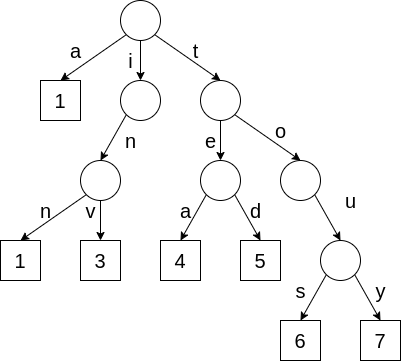
\includegraphics[width=200px]{images/8_Prefix_search/prefix_trie.png}
\end{figure}

Let's suppose we want to look for $P=te$, so we need to find the starting node, so we search for $te\$$:
\begin{itemize}
    \item we start from the root;
    \item we pick $t$;
    \item we have $e$ and $o$, we pick $e$;
    \item we have $a$ and $d$, we pick $a$ since $a \geq \$$, starting point is 4.
\end{itemize}
Now we need to find the ending point, so let's query for $te\#$:
\begin{itemize}
    \item we start from the root;
    \item we pick $t$;
    \item we have $e$ and $o$, we pick $e$;
    \item we have $a$ and $d$, we pick $d$ since is the last one $d \leq \#$, ending point is 5.
\end{itemize}
So we dropped to $O(p)$ time and $O(p)$ I/Os and depending on $p$ it can be useful than the other approaches.

To improve further of course we could build a trie over the starting elements of each block, so always using the two level indexing.

\subsection{Compacted trie}
We can compact a trie deleting the nodes with one outgoing edge and storing the whole substring from that path on the outgoing edges and storing the prefix size on the node:
\begin{figure}[H]
    \centering
    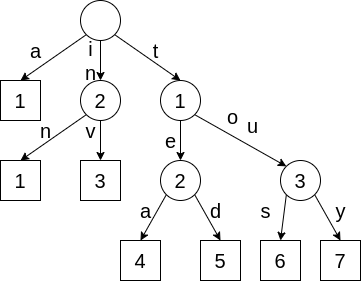
\includegraphics[width=200px]{images/8_Prefix_search/prefix_compacted_trie.png}
\end{figure}

If we want to avoid the storage of the letters, in case of long substrings we can store on the edges a triple of values: $<\text{string number}, \text{starting position}, \text{end position}>$, so for example instead of $in$ we can store $<2, 3, 3>$, so each edges has constant size!
Now the trie has size: $l + l - 1 + (2l -1) = O(l) \approx \#$strings, in which $l$ is the number of leaves.

In the end our structure to compute prefix search is:
\begin{figure}[H]
    \centering
    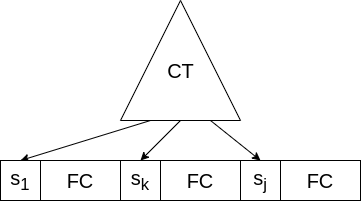
\includegraphics[width=200px]{images/8_Prefix_search/prefix_CT_and_FC.png}
\end{figure}
we need $O(p)$ I/Os at most, which is the trie traverse and the eventual string extraction since edges are compacted.

NB: if the first string of each block fits inside a block we can save I/Os trying to always use it in the tuples of compacted edges.

\section{Another 2-level index by example}
We want to design a two-level index data structure based on compacted tries and blocks of 3 strings.
In input:
\begin{itemize}
    \item aabaa, aabab, aabba;
    \item ababaaa, ababaab, abababa;
    \item abababb, ababbbb, abbaaaa;
    \item bbaba, bbabaa, bbabab;
    \item bbba, bbbab, bbbb.
\end{itemize}
We need to compress strings in block with front coding, first string of each block is kept as is, the other ones will be encoded as $<\text{prefix size}, \text{postfix}>$:
\begin{itemize}
    \item $<0, aabaa>, <4, b>, <3, ba>$;
    \item $<0, ababaaa>, <6, b>, <5, ba>$;
    \item $<0, abababb>, <4, bbb>, <2, baaaa>$;
    \item $<0, bbaba>, <5, a>, <5, b>$;
    \item $<0, bbba>, <4, b>, <3, b>$.
\end{itemize}
the compressed part goes to the disk and for the first string we build an index, assuming that we have enough space in internal memory to store first string for each block:
\begin{figure}[H]
    \centering
    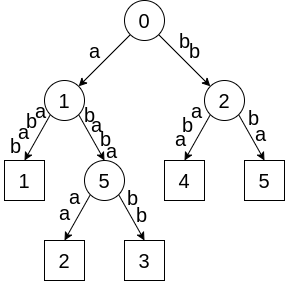
\includegraphics[width=200px]{images/8_Prefix_search/prefix_compacted_trie_example.png}
\end{figure}
we have our uncompacted trie but we can improve the memory occupancy avoiding to store the substrings and replacing them with $<$character to branch, string index, start position, end position$>$:
\begin{figure}[H]
    \centering
    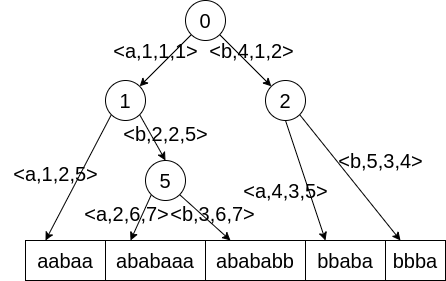
\includegraphics[width=250px]{images/8_Prefix_search/prefix_more_compacted_trie.png}
\end{figure}
So now each node is constant size which is good if strings are long, as in our case, and moreover we can estimate the occupied space:
\begin{itemize}
    \item $\#nodes < \#leaves < \frac{n}{B}$ because each node is at least binary;
    \item $\#leaves = \frac{n}{B}$;
    \item $\#edges = \#nodes + \#leaves -1 < 2 \frac{n}{B}$.

    NB: -1 because root node has no in-going edges.
\end{itemize}

Let's search for $P=abbab$:
\begin{itemize}
    \item we start from the root and choose the edge $a$ because the string starts with $a$;
    \item we decompress the edge and get $a$;
    \item second character is $b$, we check the node and there is an edge starting with $b$, so we use it;
    \item we decompress the edge and get $baba$;
    \item check for match: $baba \neq bbab$ so we have a mismatch!
    \item all strings from this edge starts with $aba$ but we are looking for $abb$ so we return iterators from between $s_3$ and $s_4$, so to start search in disk we must start from block 3.

    \item we fetch block 3, we decompress it and start checking for match;
    \item we find nothing in block 3;
    \item we know block 4 is already out of scope because it starts with $b$;
    \item so no matches!
\end{itemize}

Whether we fit strings in memory or in disk we have:
\begin{itemize}
    \item if first string is in memory: no I/Os for index traversal and a single I/O for the block found, then we pay $O(p)$ time comparison for traversing the trie and $O(B)$ time for searching in the block, so in total $O(p + B)$ time;
    \item if the first string is on the disk: $O(p+1)$ I/Os because we need to decompress each edge and $O(p+B)$ time.
\end{itemize}

\section{Patricia trie}
A patricia trie is a data structure useful to treat the prefix search problem without taking into account if the strings are in memory or on a disk.
The main idea is to drop edge labels from the compacted trie except for the first character, so for example we would have:
\begin{figure}[H]
    \centering
    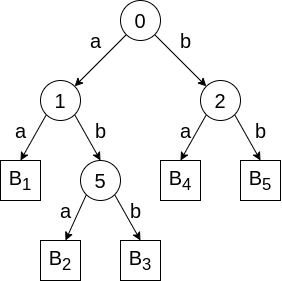
\includegraphics[width=200px]{images/8_Prefix_search/patricia_trie.png}
\end{figure}
so pointers point to the blocks and not to the strings.
It's kinda a lossy compression and we search in three phase, let's suppose we are looking for $P=abbab$:
\begin{itemize}
    \item Down-word traversal:
    \begin{itemize}
        \item we match $a$ in position 1, so we take the edge;
        \item we batch $b$ in position 2, so we take the edge;
        \item the pattern is shorter than 6 characters so we don't match. We stop the traverse and pick all the strings from this node.
    \end{itemize}
    Up to now we have no I/Os.

    \item We pick one of the strings in the result (for example $S_2$) and compute the longest common prefix:
    $$
        lcp(S_2, P) = ab
    $$
    we have a mismatch cause the ending part of $P$ $bab$ is missing.
    Moreover this information tells us that the pattern is on the right of $S_2$.
    We have 1 I/O and $O(p)$ time.

    \item Up-word traversal: we move the cursor to the next block pointed by the node we have chosen above.
\end{itemize}


